% b0, b1, b2, b3-1, b3-2, b4-1, b4-2

\section{[B-0] What's in, Doc?}

	The challenge title is quite a big hint.

	\subsection{Solution}

		Word document files (\ttt{.docx}) are actually zip files that can be extracted to reveal a bunch of XML files
		that make up the actual content of the document.

		Of course, we checked that the document didn't contain anything interesting before extracting it, which revealed
		a number of interesting files:

		\begin{listing}[!htbp]
			\begin{minted}[autogobble,xleftmargin=0.075\textwidth,xrightmargin=0.075\textwidth,frame=leftline,framesep=4mm,framerule=0.4mm]{sh}
				$ unzip test-docx.docx
				Archive:  test-docx.docx
				  inflating: [Content_Types].xml
				  inflating: _rels/.rels
				  inflating: word/document.xml
				  inflating: word/_rels/document.xml.rels
				  inflating: word/theme/theme1.xml
				  inflating: word/settings.xml
				  inflating: word/styles.xml
				  inflating: word/webSettings.xml
				  inflating: word/fontTable.xml
				  inflating: docProps/core.xml
				  inflating: docProps/app.xml
				  inflating: Light_speed_corp_logo_pink_team.xml
				  inflating: chatlog_6_may_2019.xml
			\end{minted}
		\end{listing}

		\pagebreak
		The two files that look out of place are \ttt{Light\_speed\_corp\_logo\_pink\_team.xml} and \ttt{chatlog\_6\_may\_2019.xml}.
		Opening the former reveals the flag for this challenge:

		\begin{figure}[!htbp]\centering
			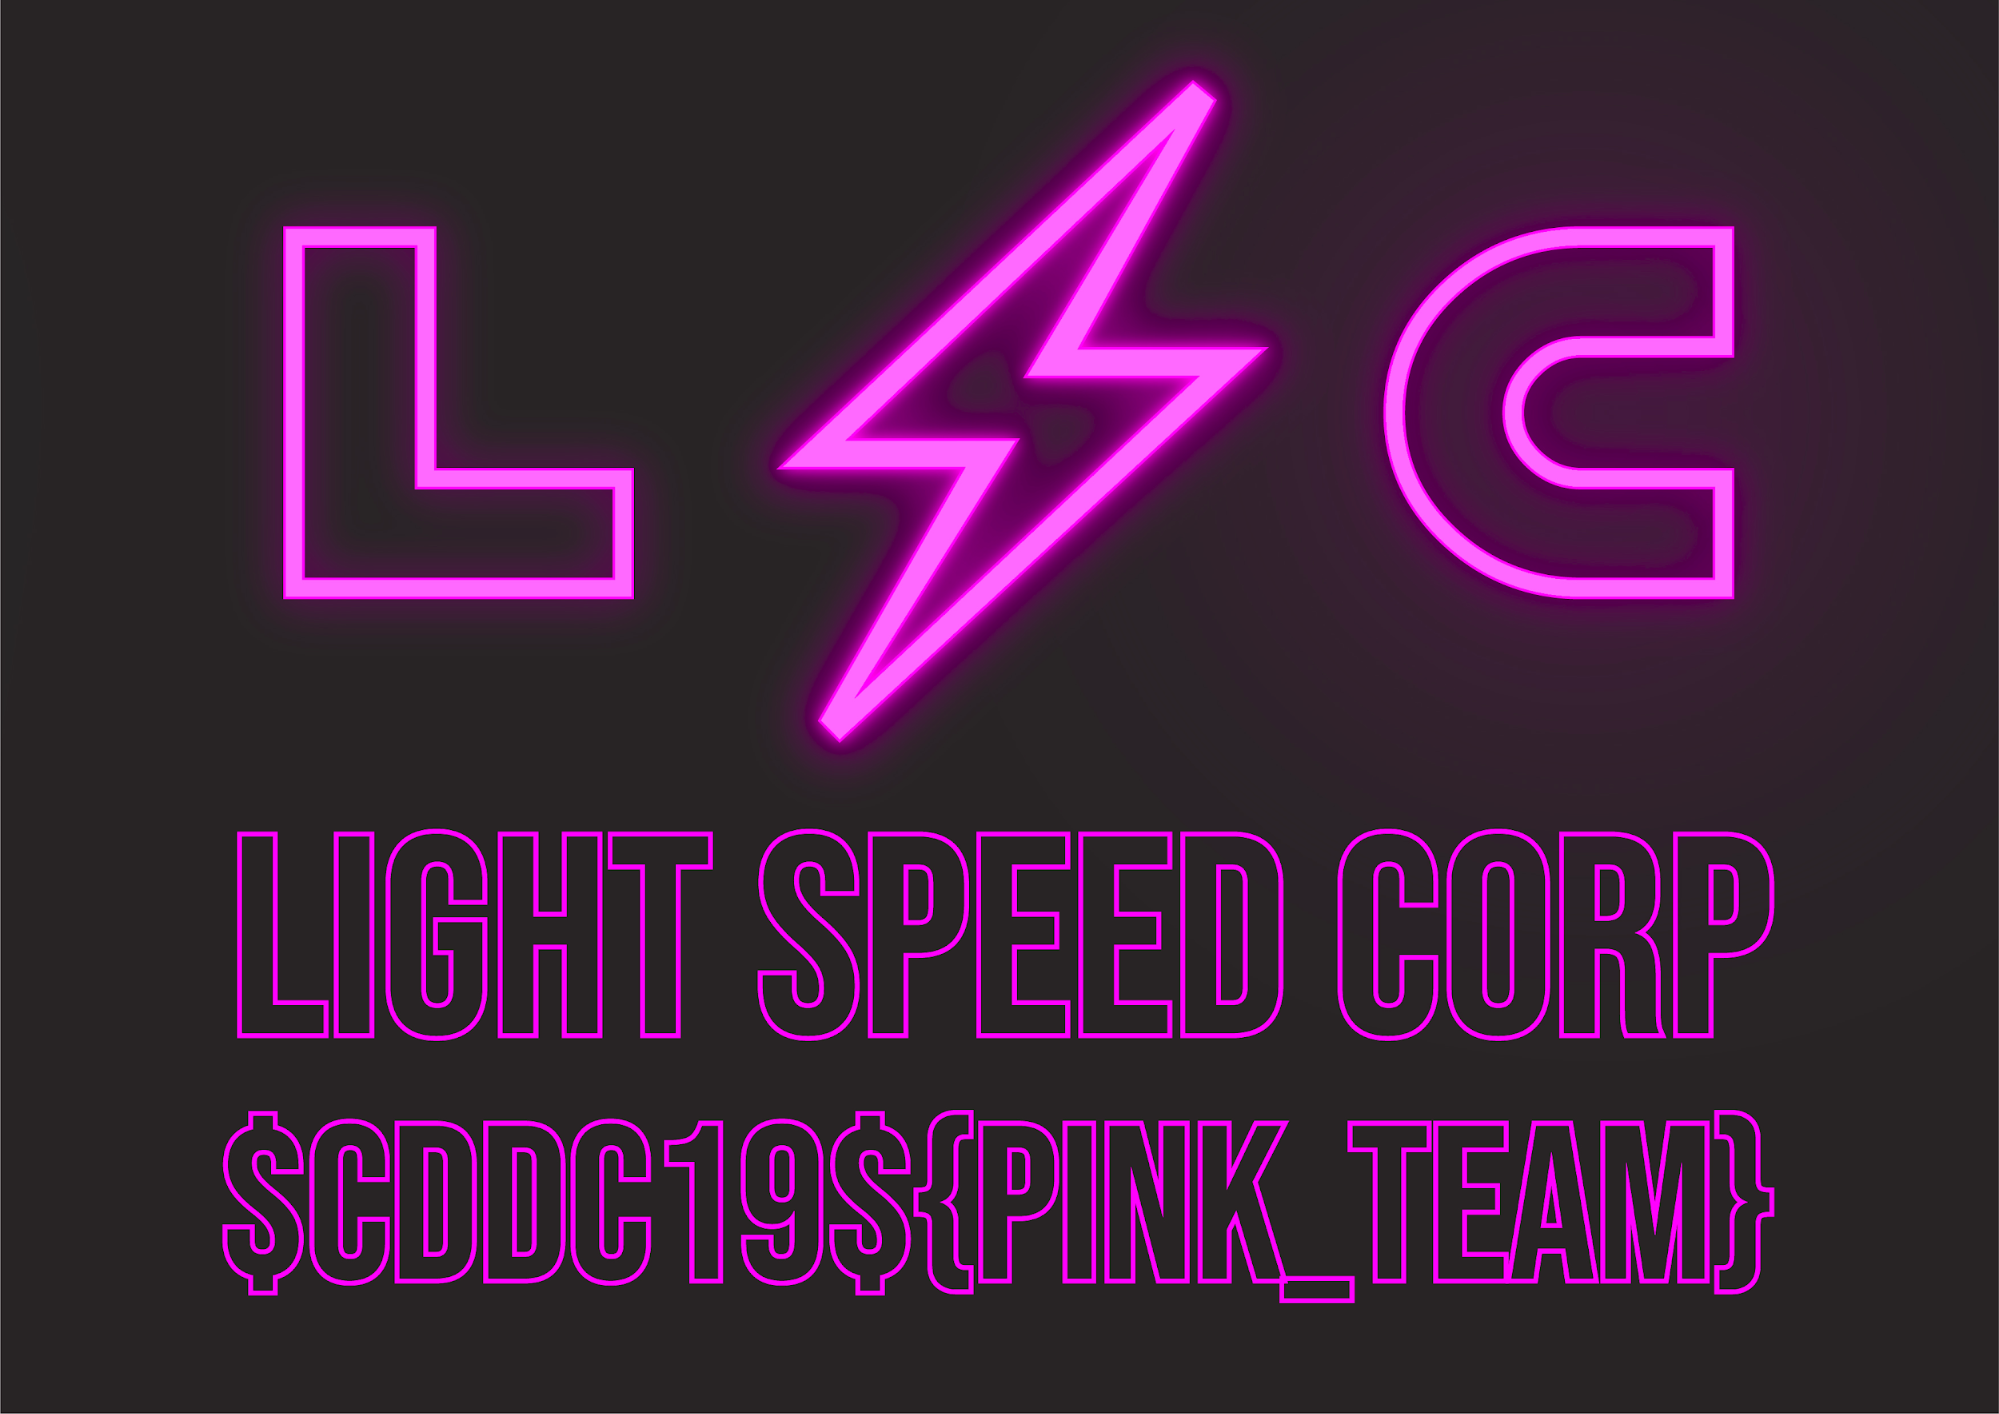
\includegraphics[width=150mm]{figures/osintblue/b0.png} \vspace{5mm}
			\caption{The flag is revealed}
		\end{figure}

		Opening the chat log reveals the usernames of our two suspicious individuals, \ttt{Caomhainn} and \ttt{kondrat\_ankudinov}.

	% end subsection

	\subsection{Flag}
		The flag for this challenge was \cddcflag{PINK\_TEAM}.
	%end subsection

% end section


\pagebreak
\section{[B-1] Fight the Binary Monster}

	An executable file, what could it be...

	\subsection{Solution}

		Disassembling Windows binaries gets quite tedious due to the Win32 functions; since the program asked for input, running strings on the
		executable gave us some good insights into the answer to its question:

		\begin{figure}[!htbp]\centering
			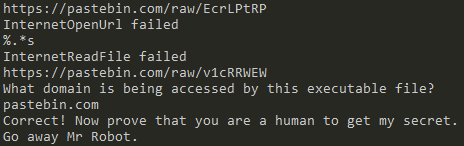
\includegraphics[width=130mm]{figures/osintblue/b1a.png} \vspace{5mm}
			\caption{Ah, pastebin my old friend}
		\end{figure}

		Dumping the output of the program when given the correct answer (\ttt{pastebin.com}) gives us a tree, and doing a post-order
		traversal gives us the flag.

		\begin{figure}[!htbp]\centering
			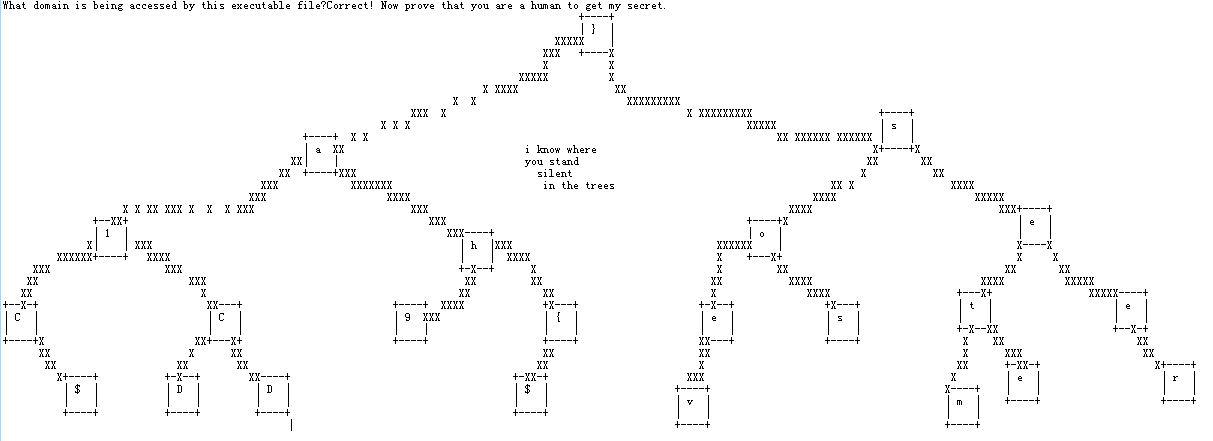
\includegraphics[width=130mm]{figures/osintblue/b1b.png} \vspace{5mm}
			\caption{Silent in the trees?}
		\end{figure}

	% end subsection

	\subsection{Flag}
		The flag for this challenge was \cddcflag{havesometrees}.
	% end subsection

% end section

\pagebreak
\section{[B-2] I <3000 PHISH}

	A macro-enabled Word document? Only slightly better than an executable...

	\subsection{Solution}
		Opening the document (without enabling the macros, of course) reveals some code (Listing \ref{code:vbaphish}). The
		key lines are reproduced below:

		\begin{listing}[!htbp]
			\begin{minted}[autogobble,xleftmargin=0.075\textwidth,xrightmargin=0.075\textwidth,frame=leftline,framesep=4mm,framerule=0.4mm]{vbnet}
				filePath = Environ("temp") + "\" + Chr(108) + "i" + Chr(103) + "h" _
					+ Chr(116) + "speed" + Chr(46) + Chr(116) + "x" + Chr(116)
				Open filePath + ":woohoo.txt" For Output As #1
			\end{minted}
		\end{listing}

		Since \ttt{:} is not a valid character in filenames in Windows, we replace it with \ttt{\_} and allow the macro
		to run, which creates a file at \ttt{lightspeed.txt\_woohoo.txt}:

		\begin{figure}[!htbp]\centering
			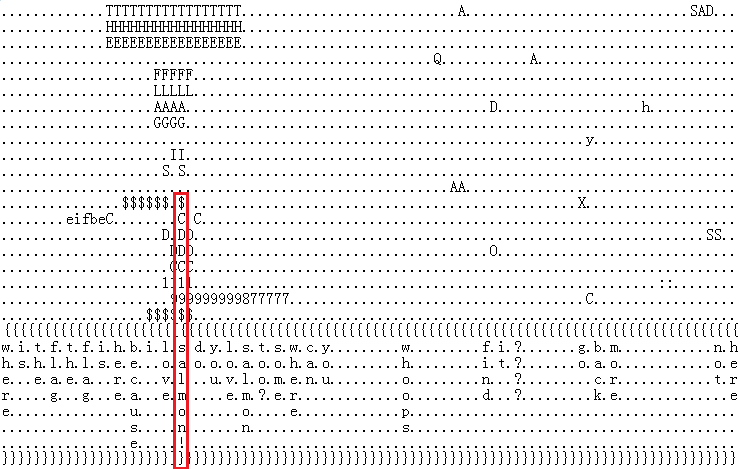
\includegraphics[width=130mm]{figures/osintblue/b2.png} \vspace{5mm}
			\caption{Vertical, sneaky}
		\end{figure}


	% end subsection

	\subsection{Flag}
		The flag for this challenge was \cddcflag{salmon!}.
	% end subsection

% end section

\pagebreak
\section{[B-3-1] Onion Sauce}

	The link given is clearly an onion site meant to be opened with the Tor browser.

	\subsection{Solution}
		Opening \ttt{ctfsg4bndpw6xurhitwa2dh66ycorghoa2ym3s3s4g3bgxqs3veaf4ad.onion} in Tor gives
		an Ethereum address \ttt{0x7bd106a84773b43e2de9f68961b53cf8fb95a1f1}, and viewing the source code of the page
		reveals a long line of \ttt{<br>} tags.

		When removed, the flag is revealed.
	% end subsection

	\subsection{Flag}
		The flag for this challenge was \cddcflag{n0W\_Y0u\_KnOw\_Th3\_S4uC3}.
	% end subsection

% end section

\pagebreak
\section{[B-3-2] When Your ZIL Turns to NIL}

	The ethereum address is found in the previous challenge, Onion Sauce.

	\subsection{Solution}

		Viewing the wallet on public blockchain explorers\footnote{\url{https://etherscan.io}} reveals that there are
		3 transactions associated with the account:

		\begin{figure}[!htbp]\centering
			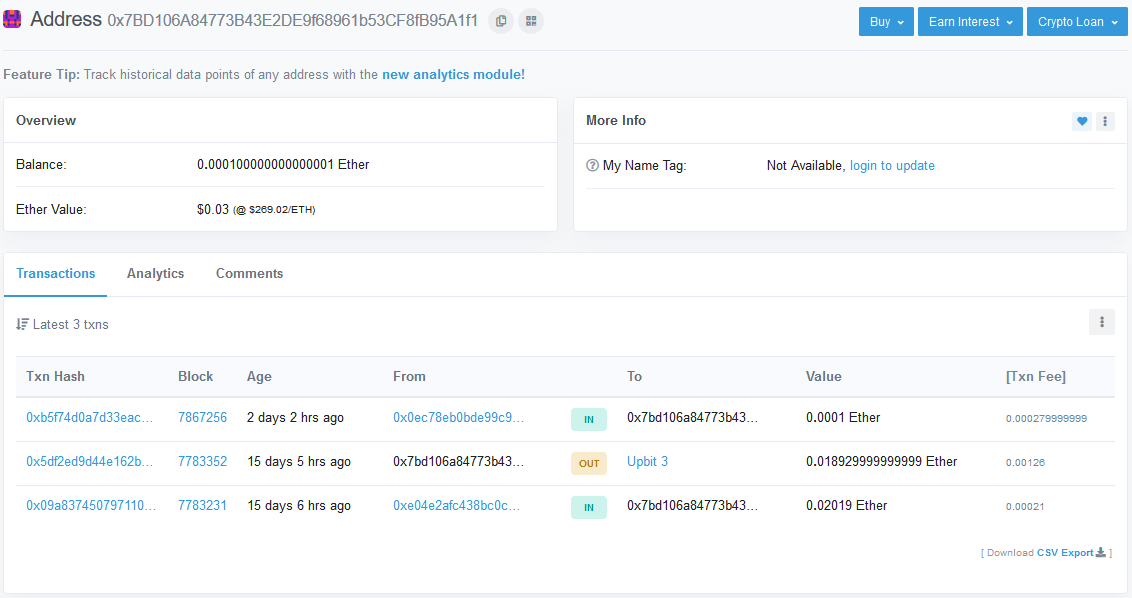
\includegraphics[width=130mm]{figures/osintblue/b32a.png} \vspace{5mm}
			\caption{Small amounts...}
		\end{figure}

		Opening the first transaction gives us the address of the victim and the amount of ethereum:

		\begin{figure}[!htbp]\centering
			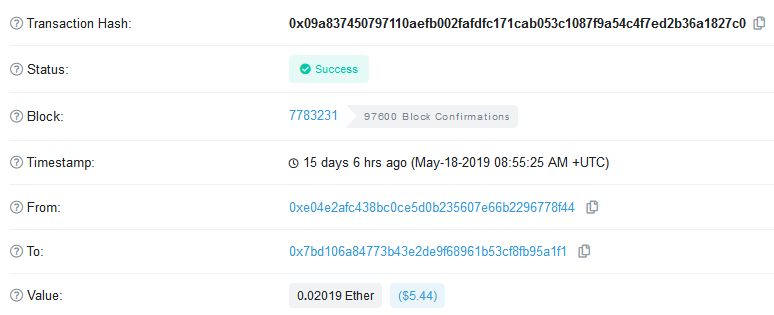
\includegraphics[width=130mm]{figures/osintblue/b32b.png} \vspace{5mm}
			\caption{The amount of ether was 0.02019}
		\end{figure}

	% end subsection

	\subsection{Flag}
		The flag is \cddcflag{0xE04E2AFC438BC0CE5D0B235607E66B2296778F44+0.02019}.
	% end subsection

% end section

\pagebreak
\section{[B-4-1] Where I Get All My GIFs From}

	The chat log from the first OSINT\_BLUE challenge gives us the names of the people we need to search for in this and the next challenge.

	\subsection{Solution}

		We got lucky and tried Twitter first, and searching \ttt{Caomhainn} gave us the culprit immediately, along with the flag:

		\begin{figure}[!htbp]\centering
			
\includegraphics[width=100mm]{figures/osintblue/b41.png} \vspace{5mm}
			\caption{Never use your real name}
		\end{figure}

	% end subsection

	\subsection{Flag}
		The flag for this challenge was \cddcflag{JEEVES\_G0T\_GIFS\_1N\_A\_J1FFY}.
	% end subsection

% end section

\pagebreak
\section{[B-4-2] Hide N Seek}

	Following on from the previous challenge, \enquote{The answer lies in this tweet}.

	\subsection{Solution}
		Following the trail of suspicious followers (made more difficult by CDDC participants following...), we arrive at this account:

		\begin{figure}[!htbp]\centering
			
\includegraphics[width=100mm]{figures/osintblue/b42.png} \vspace{5mm}
			\caption{Torvalds sounds familiar...}
		\end{figure}

		Again, the flag is clearly visible!

	% end subsection

	\subsection{Flag}
		The flag for this challenge was \cddcflag{00PS\_U\_F0UND\_ME}.
	% end subsection

% end section












